% !TeX root = ../skript.tex
% !TeX spellcheck = de_DE


\section{Lorenz-Modell}\label{lorenz-modell}

Die Gleichungen, welche das Lorenz-Modell beschreiben, enthalten viele physikalische Eigenschaften wie die Dichte, Geschwindigkeit und Temperatur der Atmosphäre. Lorenz wollte aus den bereits existierenden Gleichungen der Hydrodynamik ein Modell zur Wetterprognose erstellen. Basierend auf vorgehenden Arbeiten von Saltzman \cite{saltzman62} startete Lorenz mit den hyrodynamischen Gleichungen und verfolgte ein systematisches Näherungsvorgehen, womit er auf die drei Gleichungen stiess, die als dreidimensionales System betrachtet werden. 

Die X-Achse entspricht dabei der hydrodynamischen, räumlichen Durchschnittsgeschwindigkeit, also die durchschnittliche Konvektionsgeschwindigkeit. Die Y-Achse repräsentiert die Temperatur und die Z-Achse der Temperaturgradient. Also wie schnell sich die Temperatur verändert. Die Gleichungen lauten folgendermassen:

\begin{figure}
	\begin{align}
		\dot{x} &= \sigma(x - y)\\
		\dot{y} &= x(\rho - z) - y\\
		\dot{z} &= xy - \beta z
	\end{align}
	\caption{Gleichungen des Lorenz-Systems, Herleitung siehe Kapitel \ref{section:lorenz-modell}}
\end{figure}

Wie aus den obigen Gleichungen ersichtlich ist, sind drei Parameter vorhanden. Alle sind immer positiv.

\subsubsection{1. Parameter: $\sigma$}
$\sigma$ entspricht der dimensionslosen Prandtl Zahl. Diese ist das Verhältnis von \textit{Viskosität} und der \textit{Wärmeleitfähigkeit}. Da beide Eigenschaften die Einheit $\frac{\text{m}^2}{\text{s}}$ haben, resultiert daraus eine dimensionslose Zahl.

\subsubsection{2. Parameter: $\rho$}
Dieser Parameter ist nach dem Physiker Baron Rayleigh benannt worden und heisst Rayleigh Zahl. Es entspricht dem Verhältnis von \textit{Wärmeausdehnung} und der \textit{Viskosität}.

\subsubsection{3. Parameter: $\beta$}
Das $ \beta $ entspricht der \textit{Wärmeausdehnung}. Dabei handelt es sich um die Veränderung der geometrischen Abmessungen (Länge, Flächeninhalt und Volumen) eines Körpers, die sich mit erhöhter Temperatur vergrössern.

\begin{figure}
	\centering
	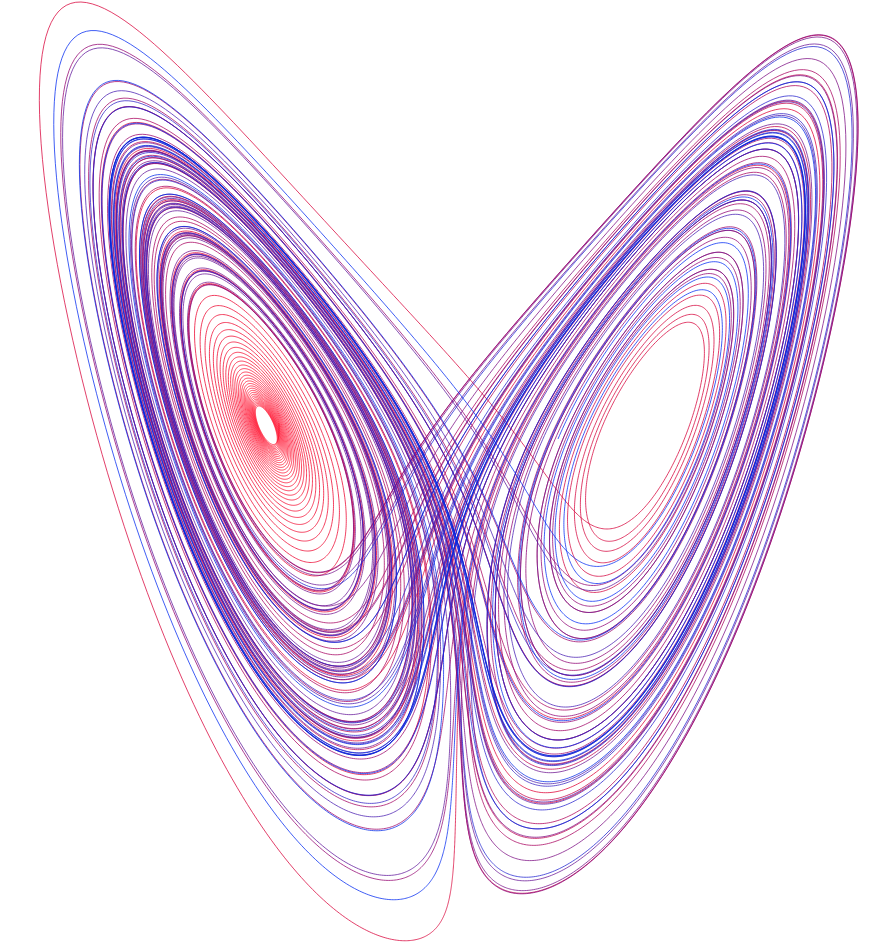
\includegraphics[width=0.3\linewidth]{lorenz/assets/lorenz-modell/lorenz-modell}
	\caption{Bahn des Lorenz-Modell mit $\rho = 28$, $\sigma = 10$ und $\beta = \frac{8}{3}$}
	\label{fig:lorenz-modell}
\end{figure}


\subsection{Numerische Lösungen}
Es gibt für das Lösen von Differentialgleichungen zwei Ansätze. Zum einen der analytische Ansatz, der eine allgmeingültige Lösung sucht. Es handelt sich bei den drei Lorenz-Gleichungen um nicht-lineare Differentialgleichungen, welche analytisch nicht lösbar sind. Aus diesem Grund fällt dieser Lösungsweg weg. 

Der zweite Ansatz ist, eine \textit{Diskretisierung} vorzunehmen und den Computer für jeden definierten Zeitpunkt die Resultate der Gleichungen \textit{numerisch} ausrechnen zu lassen. Dies ist auch der in dieser Arbeit gewählte Weg, der im Folgenden bis zur tatsächlichen Visualisierung genauer beschrieben wird.

Differentialgleichungen beschreiben die Änderungsrate der Variablen $ X, Y, Z $. Sie sagen nichts über die X-Achsen-Verschiebung der Werte aus. Aus diesem Grund kennt man die absolute Werte nicht und kann auch keine andere Werte davon ableiten. Der numerische Algorithmen können lediglich die anderen Werte ausrechnen von einem definierten Startwert. Im Abschnitt \ref{euler-verfahren} Euler-Verfahren werden wir weiter auf die Wahl des Startwertes eingehen.

\subsubsection{Euler-Verfahren} \label{euler-verfahren}

Wir wählten für die Diskretisierung das \textit{Euler-Verfahren} zur Annäherung der Werte des Lorenz-Modells. Das resultierende Gleichungssystem besteht aus einfachen Arithmetik-Operationen und ist für einen Computer einfach berechenbar. Dies erlaubt auch \textit{Smartphones} die Visualisierung effizient zu berechnen und flüssig anzuzeigen.

Das Euler-Verfahren ist ein Algorithmus der Familie der Einschritt-Verfahren. Diese Verfahren rechnen iterativ in einer Schleife die Werte von einem bekannten Startwert aus. Als nächster Ausgangspunkt wird dann das Ergebnis der vorherigen Iteration genommen und mithilfe der Differentialgleichung die Änderung bestimmt. 

Einschritt-Verfahren brauchen einen Startwert, von wessen sie die nächsten Ausgangspunkte ausrechnen können. Wir haben im Rahmen dieses Berichtes keine Optimierung des Startwertes durchführen können, sondern einfach eine sinnvolle Annahme getroffen. Dieser Anfangswert war konstant und fester Teil des Algorithmus, den wir modeliert haben.

Wir begannen zuerst mit dem Startwert $ P(0, 0, 0) $. In den anschliessenden Untersuchungen des Algorithmus zeigte sich, dass dieser Startwert zugleich eine Lösung des Lorenz-Systems ist. Aus diesem Grund hat sich das Model auf den Ursprung stabilisiert. Wir entschieden uns den Startwert auf $ P(0.1, 0.1, 0.1) $ zu verschieben, dieser Wert ist keine Lösung des Lorenz-Systems und das Modell stabilisierte sich nicht mehr.

Als Basis für das Euler-Verfahren verwenden wir den Differenzenquotient $ \frac{dx}{dt} \approx \frac{x_{n + 1} - x_n}{\Delta t} $ \cite{dahmen2008}.  Weil wir den nächsten Punkt im 3D-Raum ausrechnen möchten, formen wir die Gleichung zu $ x_{n + 1} $  um und rechnen sie für alle Achsen getrennt aus.

\begin{align}
    x_{n + 1} &= x_n + \frac{dx}{dt} \cdot \Delta t\\
    y_{n + 1} &= y_n + \frac{dy}{dt} \cdot \Delta t\\
    z_{n + 1} &= z_n + \frac{dz}{dt} \cdot \Delta t
\end{align}

% TODO Neuschreiben, detailhafter
Für die Ableitungen können wir nun die Gleichungen des Lorenz-Modells einsetzen.
\begin{align}
    x_{n + 1} &= x_n + \sigma(x_n - y_n) \cdot \Delta t\\
    y_{n + 1} &= y_n + x_n(\rho - z_n) - y_n \cdot \Delta t\\
    z_{n + 1} &= z_n + (x_n \cdot y_n - \beta \cdot z_n) \cdot \Delta t
\end{align}

Dieses System entspricht dem Code der Visualisierung weiter unten. Im Differentialterm wurde die Differentialgleichung des Lorenz-Modells eingesetzt.
